\newpage
\section{Relative Güte der Features}
Der Featurevektor besteht in seiner ungekürzten Form aus 261 Features. Im J48 Klassifizierer wird beim Aufbau des Entscheidungsbaumes jedes Feature als mögliche Alternative für jeden Knoten im Baum in Betracht gezogen. Hierdurch entsteht eine hohe Laufzeit. Es ist möglich, die Auftrittshäufigkeiten von Featurs im Entscheidungsbaum zu ermitteln und so Features zu identifizieren, die für den Klassifizierer viele Informationen liefern. Dazu werden zufällige Untermengen der Trainingsmenge erzeugt, in denen die Klassenverteilung erhalten bleibt. Mit jeder Untermenge wird anschließend ein Klassifizierer trainiert. Die entstandenen Entscheidungsbäume der Klassifizierer werden dann durchlaufen und für jedes Feature wird die Anzahl der Vorkommen im Entscheidungsbaum gespeichert. Features, die viele Informationen für den Klassifizierer liefern, kommen häufiger im Baum vor als andere.

\begin{figure}[H]
    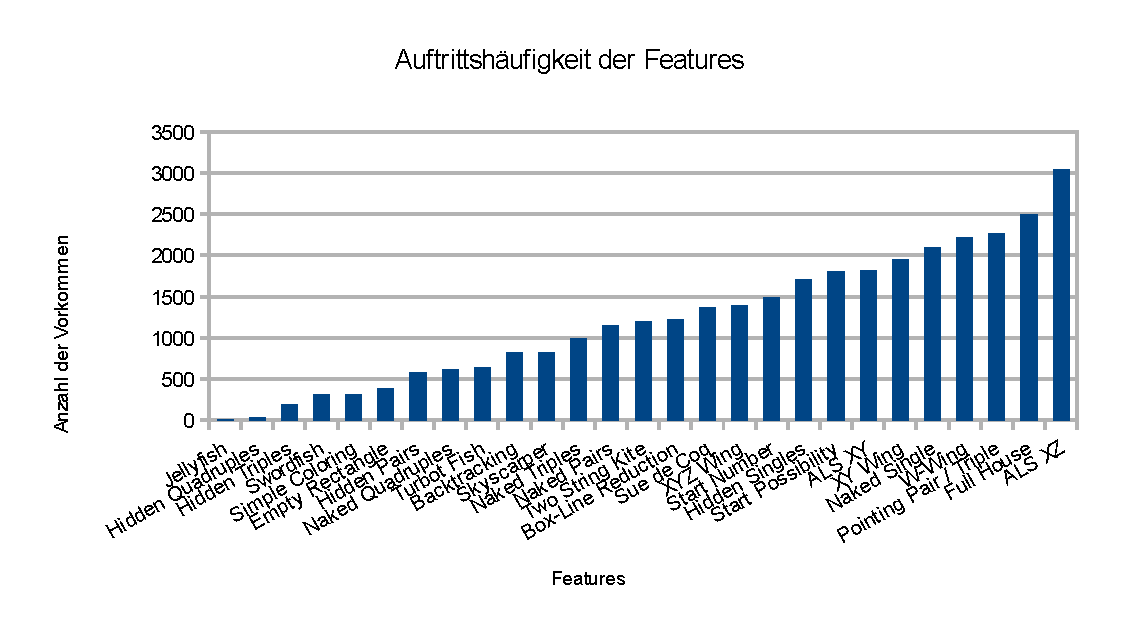
\includegraphics[width=\textwidth,height=\textheight,keepaspectratio]{./img/features.eps}
    \caption{Auftrittshäufigkeit der Features}
\end{figure}

\noindent Das Ergebniss der Analyse von 1000 Klassifizierern mit verschiedenen Untermengen ist in \textbf{Abbildung 5.9} dargestellt. Um die Grafik übersichtlicher zu gestalten sind hier alle Features nach den Lösungsmethoden gruppiert und nicht nach der Ziffer aufgeteilt. Zusätzlich sind sie nach ihrer Auftrittshäufigkeit aufsteigend sortiert. Hier sieht man sehr eindeutig, dass einige Features um ein Vielfaches häufiger Vorkommen als andere. Daher ist ihr Informationsgehalt für den Klassifizierer höher.\\
Jede Lösungsmethode steuert neun Features zum Featurevektor bei. Das gilt auch für die am Anfang vorgegebenen Ziffern und die von Anfang an vorhandenen Möglichkeiten. Wie in Kapitel \ref{Entkopplung} erklärt, sind alle dieser neuer Blöcke nach ihrer Häufigkeit sortiert. Die ersten Einträge dieser neuner Blöcke enthalten in der Regel aussagekräftigere Informationen, da oft der Fall auftritt, dass die hinteren Einträge null sind. Dies soll am Beispiel der Methode \textit{ALS XZ} verdeutlicht werden.

\begin{figure}[H]
    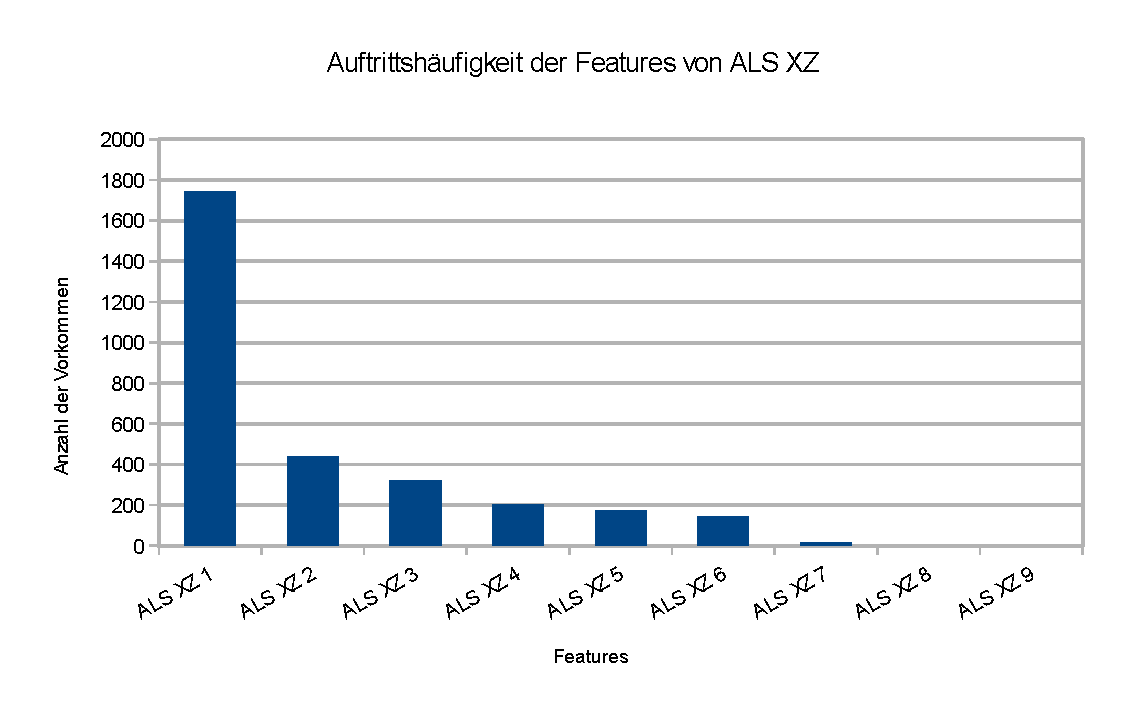
\includegraphics[width=\textwidth,height=\textheight,keepaspectratio]{./img/alsxz_anzahl.eps}
    \caption{Auftrittshäufigkeit der Features der Lösungsmethode \textit{ALS XZ}}
\end{figure}

\noindent In \textbf{Abbildung 5.10} sieht man, dass die Features, die, nach der Sortierung nach der Häufigkeit, die höheren Werte repräsentieren, auch öfter im Baum auftreten. Daraus lässt sich schließen, dass diese Features relevantere Informationen für den Klassifizierer darstellen. Die hinteren Features sind, selbst bei der am häufigsten auftretenden Methode, vernachlässigbar.\\
In Weka ist der CFS\footnote{Correlation based Feature Selection} Algorithmus implementiert. Dieser beruht auf der Annahme, dass gute Features eine starke Korrelation zur Klasse aufweisen, aber untereinander eine schwache Korrelation haben. \cite{Hall1998}. Lässt man diesen Algorithmus die besten Features auswählen, dann erhält man folgende Liste.
\begin{itemize}
\item Hidden Singles 1
\item Pointing Pair / Triple 1
\item Pointing Pair / Triple 2
\item Pointing Pair / Triple 3
\item Naked Pair 1
\item Naked Triple 1
\item Naked Quadruple 1
\item Hidden Pair 1
\item W Wing 1
\item XY Wing 1
\item XYZ Wing 1
\item Skyscarper 1
\item Two String Kite 1
\item Sue de Coq 2
\item ALS XZ 0
\item ALS XZ 1
\item ALS XY 0
\end{itemize}
An der Auswahl kann man erkennen, dass auch bei diesem Algorithmus Features bevorzugt werden, die, nach der Sortierung nach der Häufigkeit, die höheren Werte repräsentieren. Ansonsten deckt sich, bis auf die Bevorzugung der Methode \textit{Pointing Pair / Triple}, das Ergebniss fast mit der Analyse der Auftrittshäufigkeit. Auffallend ist hier, dass weder die Anzahl der am Anfang bekannten Zahlen noch die Anzahl der am Anfang wählbaren Positionen ausgewählt wurden. Die relevantesten Informationen über den Schwierigkeitsgrad eines Sudokus lassen sich demnach aus den verwendeten Lösungsmethoden ziehen. Dies ist eventuell bedingt dadurch, dass das Einteilungsverfahren für die Testsudokus ebenfalls auf den verwendeten Lösungsmethoden beruht. Um das zu untersuchen, benötigt man ein Testset, das von menschlichen Spielern bewertet wurde.\\
Wenn man nun die gleichen Lösungsmthoden verwendet, um die Sudokus zu lösen, aber nur die Features im Featurevektor abspeichert, die vom CFS Algorithmus als relevant identifiziert wurden, dann liegt die Klassifikationsgenauigkeit bei 77,98\% statt zuvor bei 79,8\%. Man verliert also 1,82\% Genauigkeit in der Klassifikation, der Featurevektor enthält aber dafür weniger als 7\% der ursprünglichen Features.